\chapter{Results}
    Results from the simulation and the Deep Q Learning Controller will be covered in this chapter. First we will go through the leg patterns to see how they move and how accurate they are with previous experiments. Then we will focus on the robot displacement and the simulation. Finally results of the controller will be presented.
    
    \section{Leg patterns}\label{sec:res_legs}
        This is the basic results needed in order to build the other modules. We need to be able to encode the ten sequences that a multistable joint can have as seen on Figure \ref{fig:sequences}. We will go through the sequences here. Each time we will have the same structure, a Figure on the left representing the final state machine or the order of motion from the middle and the top block, which can vary from forward and backward movement. On the right we will have a Figure which plot the position of the leg in x-axis and z-axis with respect to the position off the actuator represented by the colorbar.
        \begin{figure}[h]
            \centering
            \begin{subfigure}{.2\textwidth}
            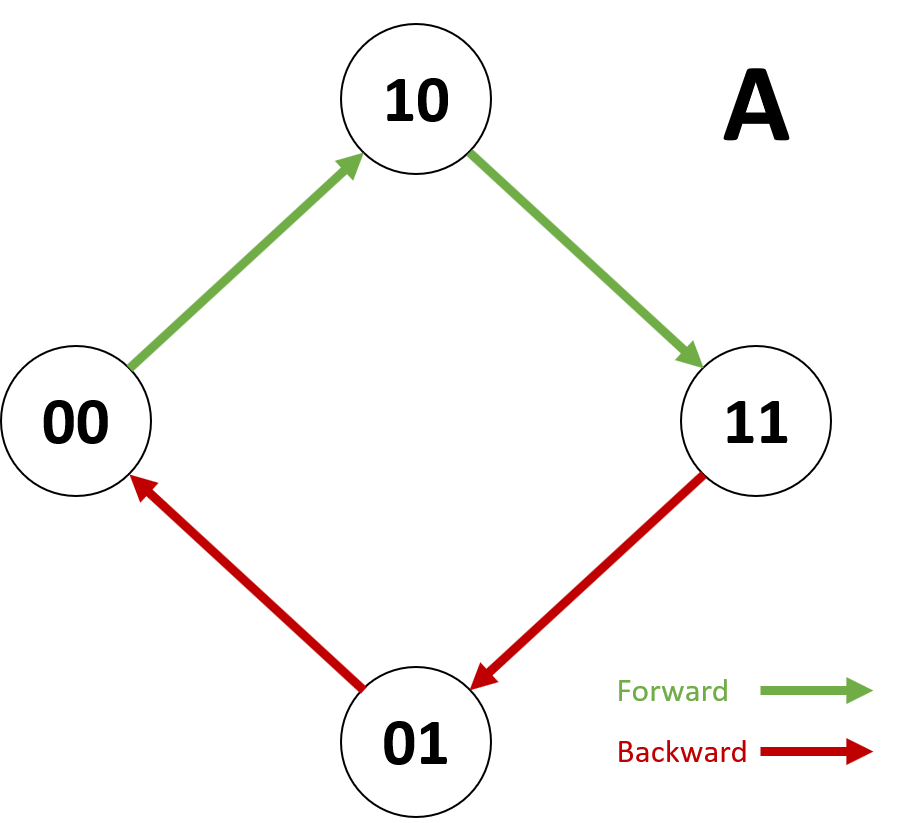
\includegraphics[width=\textwidth]{images/S_A.png}
            \end{subfigure}%
            \begin{subfigure}{.6\textwidth}
            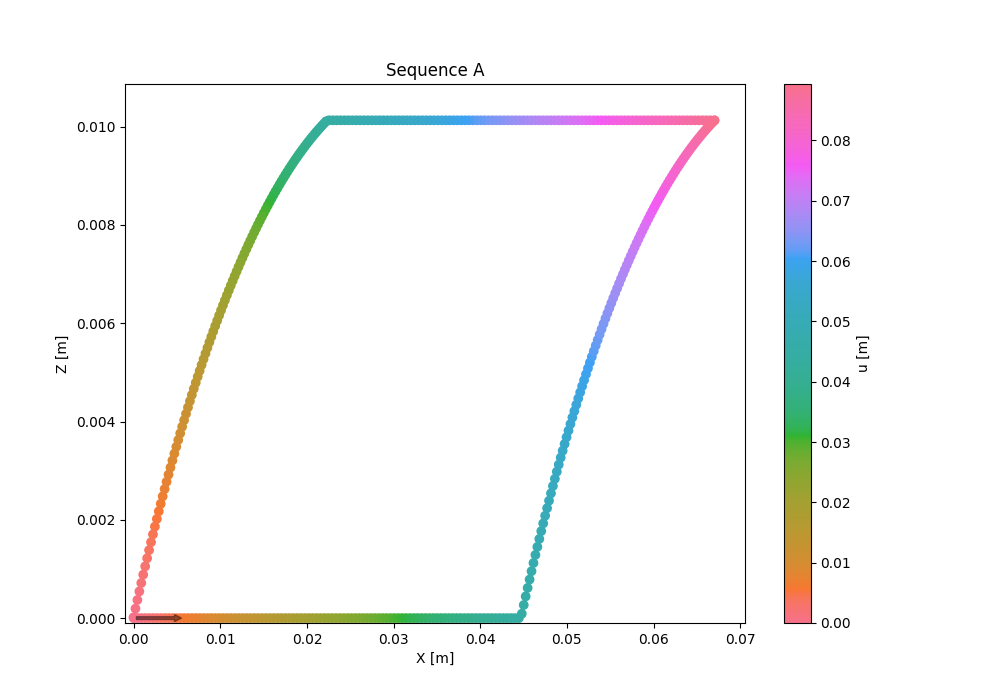
\includegraphics[width=\textwidth]{images/A.png}
            \end{subfigure}
            \caption{Sequence A is one of the simplest sequence where the middle block moves first in forward and backward motion. This leads to a hysteresis as we can see. The arrow shows the direction of motion, which is counter-clockwise. Sequence B (Figure \ref{fig:appendix_seq_B}) is identical except that it goes clockwise.}
        \end{figure}
        
        
        \begin{figure}[h]
            \centering
            \begin{subfigure}{.2\textwidth}
            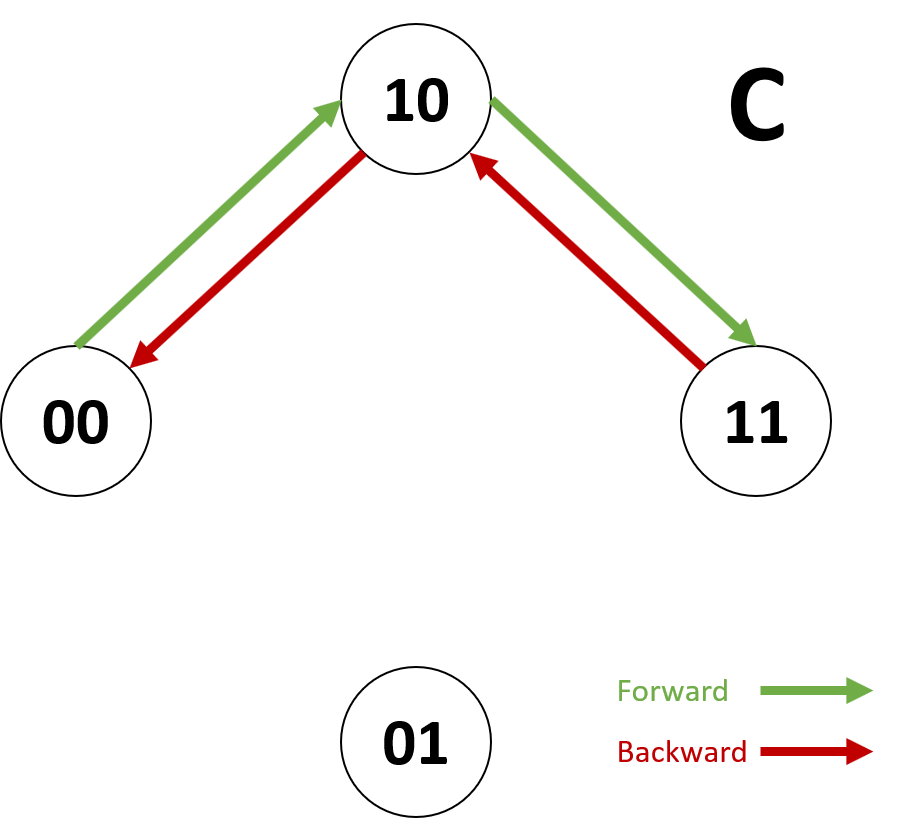
\includegraphics[width=\textwidth]{images/S_C.png}
            \end{subfigure}%
            \begin{subfigure}{.6\textwidth}
            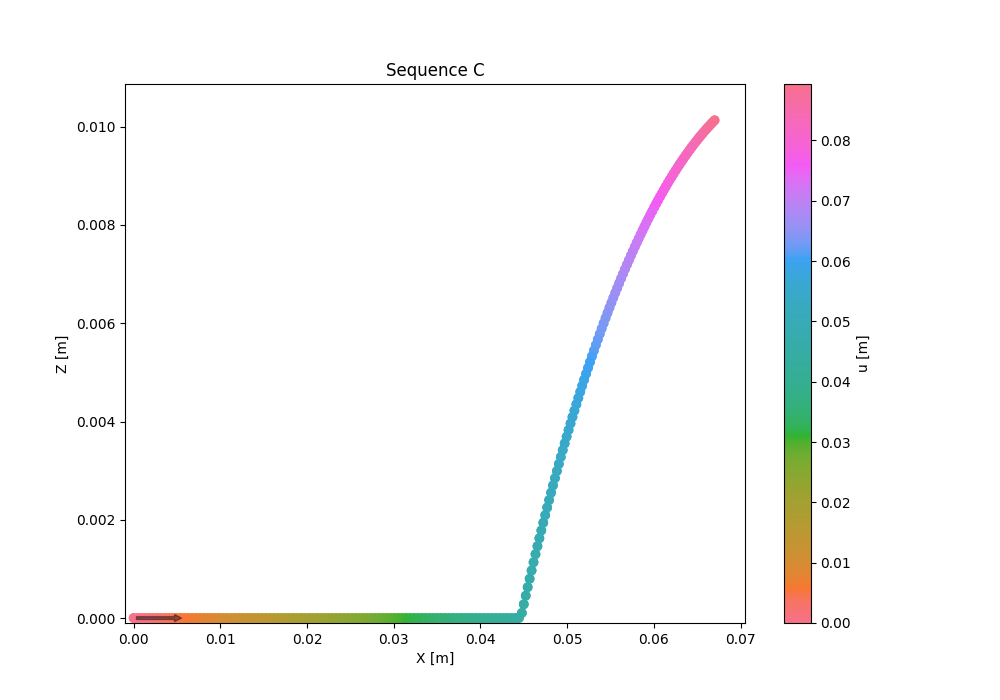
\includegraphics[width=\textwidth]{images/C.png}
            \end{subfigure}
            \caption{Sequence C is a symmetrical sequence where the forward and backward motion are following the same path. In this sequence the middle block moves first during the forward motion and the top block moves first during the backward motion. Sequence D (Figure \ref{fig:appendix_seq_D}) is very similar.}
        \end{figure}
        
        \begin{figure}[h]
            \centering
            \begin{subfigure}{.2\textwidth}
            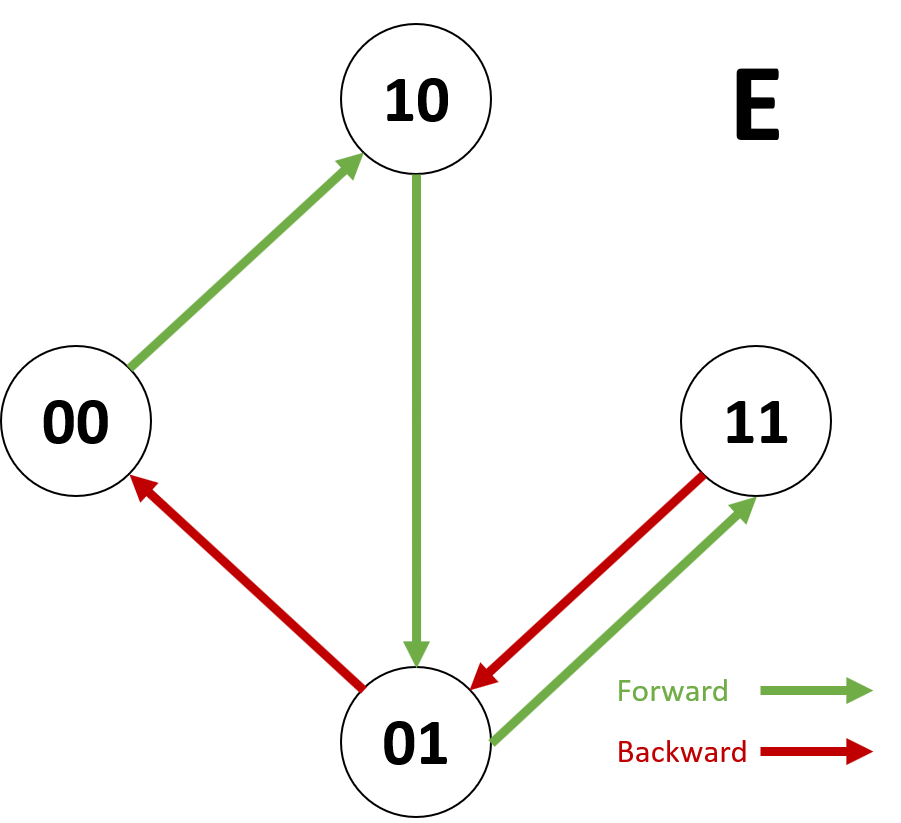
\includegraphics[width=\textwidth]{images/S_E.png}
            \end{subfigure}%
            \begin{subfigure}{.6\textwidth}
            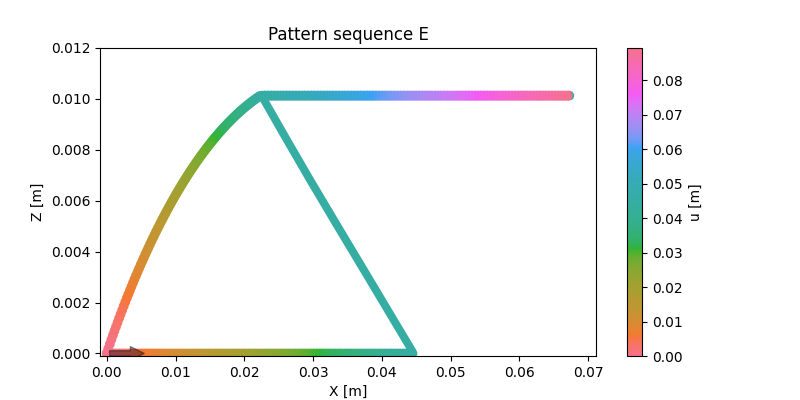
\includegraphics[width=\textwidth]{images/E.png}
            \end{subfigure}
            \caption{Sequence E is the first sequence with a avalanche mechanism where two blocks swap positions. This happens in the middle of the forward motion. We can see that after moving horizontally, both legs switch their position without any input from the actuator, producing this triangle shape. Sequence F (Figure \ref{fig:appendix_seq_F} is performing similarly.}
        \end{figure}
        
        \begin{figure}[h]
            \centering
            \begin{subfigure}{.2\textwidth}
            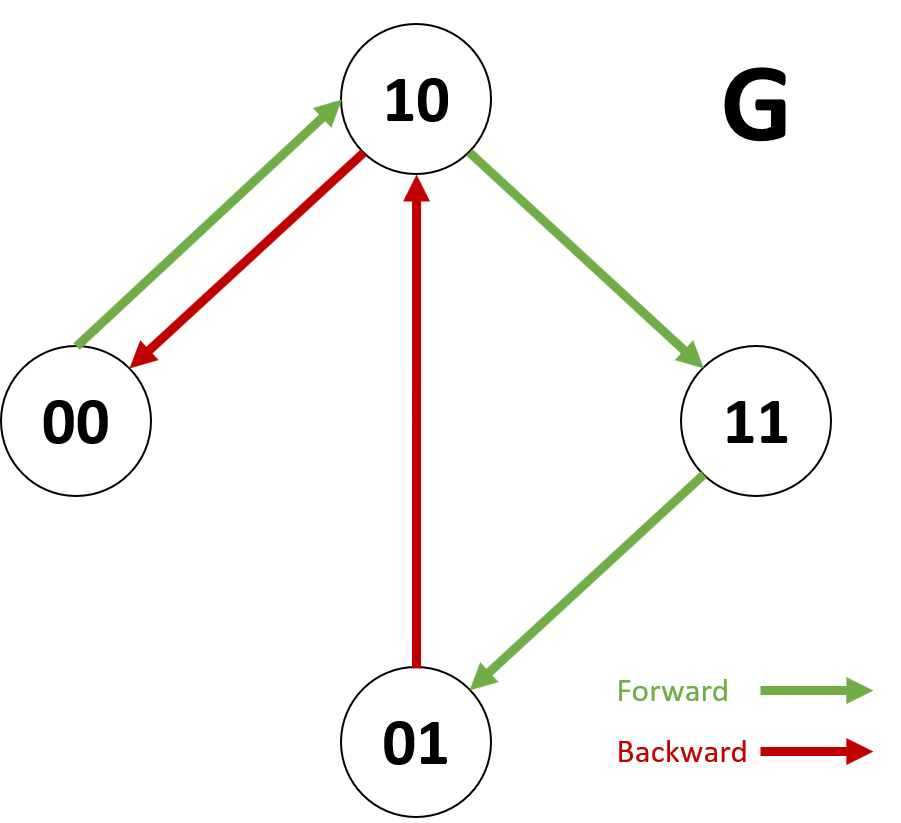
\includegraphics[width=\textwidth]{images/S_G.png}
            \end{subfigure}%
            \begin{subfigure}{.6\textwidth}
            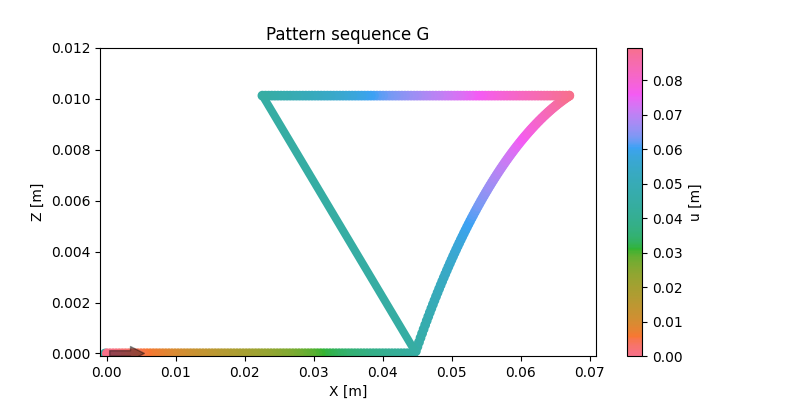
\includegraphics[width=\textwidth]{images/G.png}
            \end{subfigure}
            \caption{Sequence G is similar to sequence E and F as there is also an avalanche effect that swap two blocks positions. But this time the swap occurs during backward actuation instead of forward actuation. Sequence H (Figure \ref{fig:appendix_seq_H} is performing similarly.}
        \end{figure}

        \begin{figure}[h]
            \centering
            \begin{subfigure}{.2\textwidth}
            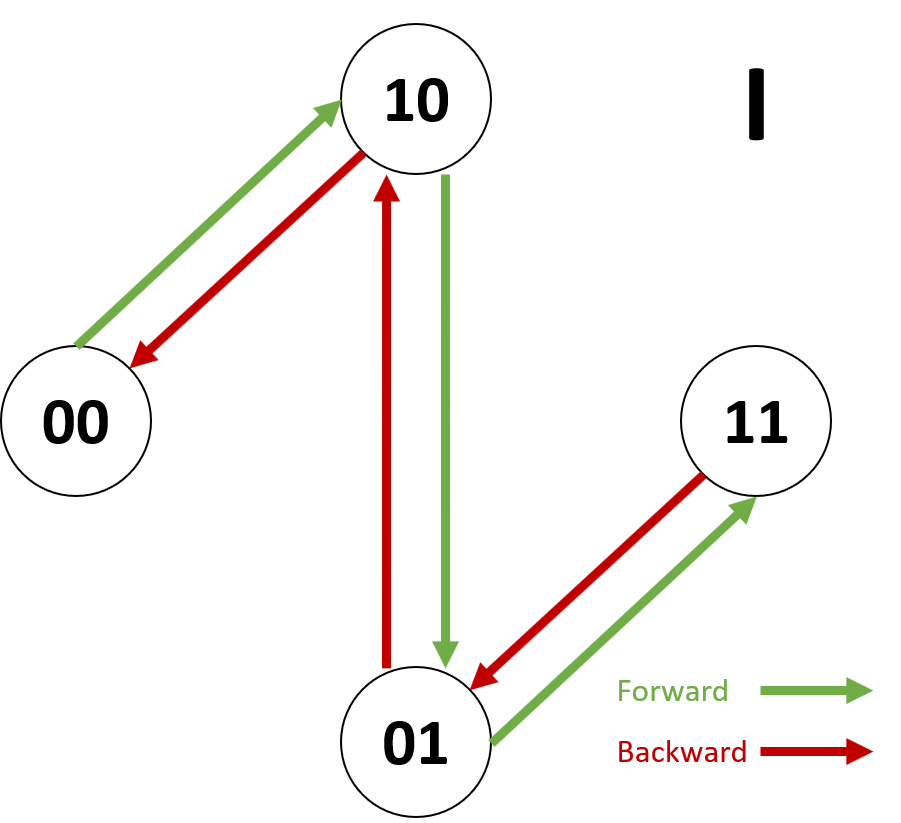
\includegraphics[width=\textwidth]{images/S_I.png}
            \end{subfigure}%
            \begin{subfigure}{.6\textwidth}
            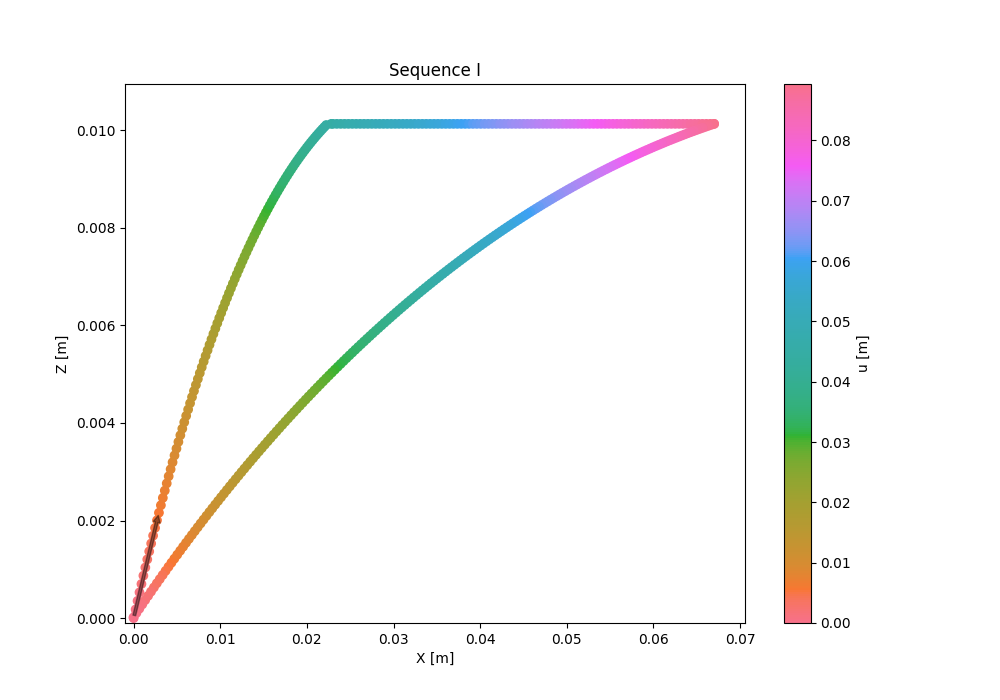
\includegraphics[width=\textwidth]{images/I.png}
            \end{subfigure}
            \caption{Sequence I is a sequence with two avalanches mechanisms. This time the two blocks swap positions during forward and backward motions.}
        \end{figure} 
        
    \section{Robot behavior visualization}
        Let's show what information are provided in the simulation's video. There is an example of the type of information as a result in Figure \ref{fig:drawing}. The simulation represents the robot in a schematic top view way, with a main frame represented by yellow blocks. On each corner there is a multistable joint as for the real robot. Actuators are not directly represented but they are linked to two type of top blocks, green ones and magenta ones. Top blocks with the same color are linked together to the same actuator. Linking the blocks together we have springs and arms, respectively in gray and red colors
        
        \begin{figure}[h]
            \centering
            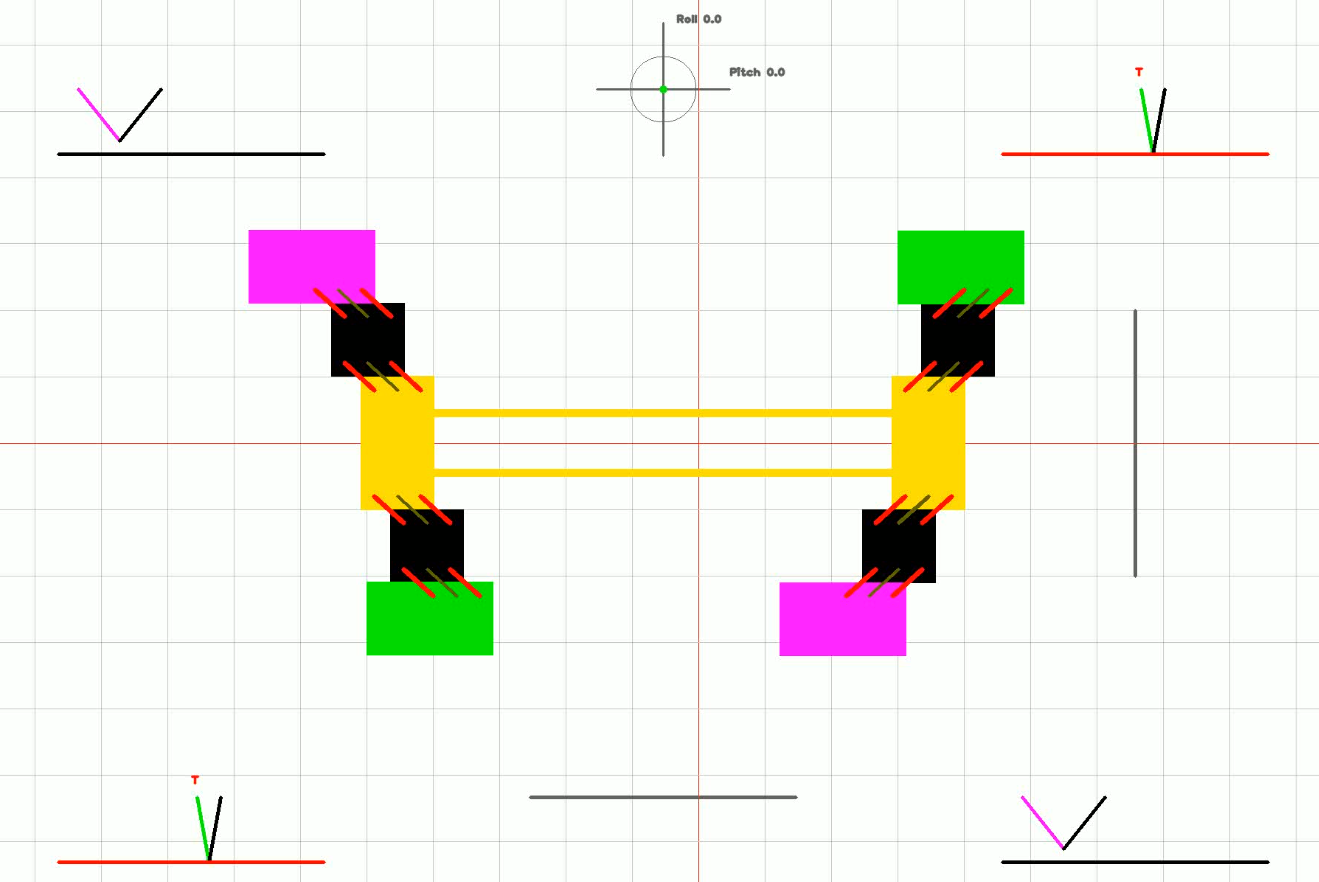
\includegraphics[width=0.8\textwidth]{images/drawing.png}
            \caption{An example of the type of drawing the simulation produces. It is mainly a top view of the robot, with the frame in yellow, and the four multistable joints at each corner of the main frame. The actuators are not represented directly but can be determined with top blocks that are connected together by color. On the four corners there is a side view of the corresponding leg, with an horizontal line that represent the ground relative to the foot. This line is in black when the foot is not touching the floor, and in red when it is touching. On the top of the image, there is a representation of the pitch and roll angle of the main frame relative to the ground. this is also duplicated with the vertical line on the right and the horizontal line on the bottom of the picture, which represent a front side view of the robot. The background of the image consists of a grid with a reference of the origin with a red cross. It is used to visualize how the robot moves relative to the ground.}
            \label{fig:drawing}
        \end{figure}
        
        The view of the robot is a top view as it allows us to understand how the sequences are moving. There are have four smaller views on the image's corners. Those views represent a side view of each multistable joint. For example the bottom left leg, there is a horizontal line which is a virtual representation of the ground position relative to this leg. There are also green and black lines, the green line represent the arm that link the green block to the leg endpoint. The black line represents the arm that link the black block to the leg endpoint. The text (e.g. \textit{J1}) tells which leg it is, and the red line is present when the leg is in contact with the ground. In the Figure case, there are two (green) legs are touching the ground while two others (magenta) are not.\\
        
        On top of the image there is a cross with a green dot. This is one way to represent the attitude of the robot, in particular the pitch and roll rotation. Pitch rotation will be positive when the front of the robot (on the right) is lower than the rear of the robot (on the left). Similarly for the roll axis. There is also a second representation of the inclination of the robot with a vertical line on the right of the image that will be tilted with the roll angle and the horizontal line on the bottom of the image that represent the pitch angle.\\
        
        On the background of the image there is a grid in gray to see how the robot is evolving compare to the ground. And to have a reference there is a red cross in the background that represent the origin of the virtual world. The grid size can be configured in the JSON file. 
        
    \section{Robot trajectory}\label{sec:res_position}
        The simulation also output a graph with the trajectory and orientation of the robot. A shown on Figure \ref{fig:robot_position}, there are the x-axis and y-axis displacement of the robot on the first subplot and the orientation change in the second subplot, this correspond to the heading of the robot. The horizontal axis is the actuation in a specific unit, which is in cycles. The plot also gives information for the final values of the cycle, in this case, a displacement of $-9cm$ for the x-axis, $0.2cm$ for the y-axis and no orientation change after a cycle.
        \begin{figure}[h]
            \centering
            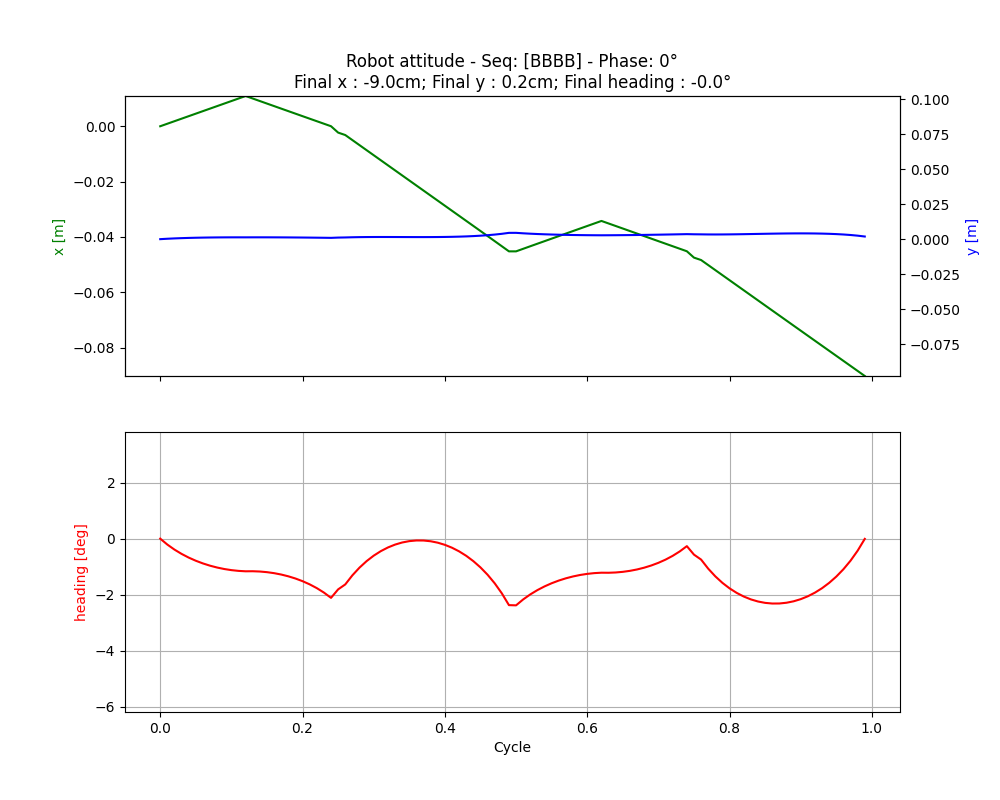
\includegraphics[width=0.7\textwidth]{images/robot_position.png}
            \caption{An example of output produced by the simulation that tracks the trajectory and the orientation of the robot during the cycles.There is the x-axis displacement (horizontal in videos) and the y-axis displacement (vertical in videos). Also the orientation change of the robot is plotted, which correspond to the heading. This plot has been generated using sequence \textit{BBBB} with a phase difference of $0$°}
            \label{fig:robot_position}
        \end{figure}
    
    \section{Displacement mapping}\label{sec:res_mapping}
        With the simulation and its parameters a mapping table can be created with all the possibles motion for the robot. Each leg can be programmed to act with one of the 10 sequences and the actuators can have a phase difference of 0° or 180°. This gives $20'000$ combinations. To create a correct symmetry we also need to switch the starting position of the actuators, which gives a total of $40'000$ combinations. Each combinations will produce a x-axis and a y-axis displacement for the robot and a change in orientation that we can represent in a row. The table produced contain then $40'000$ rows and $6$ columns containing the sequence, actuation phase and starting point as input and the displacement of the robot (x, y, heading).\\
        
        \begin{figure}[h]
            \centering
            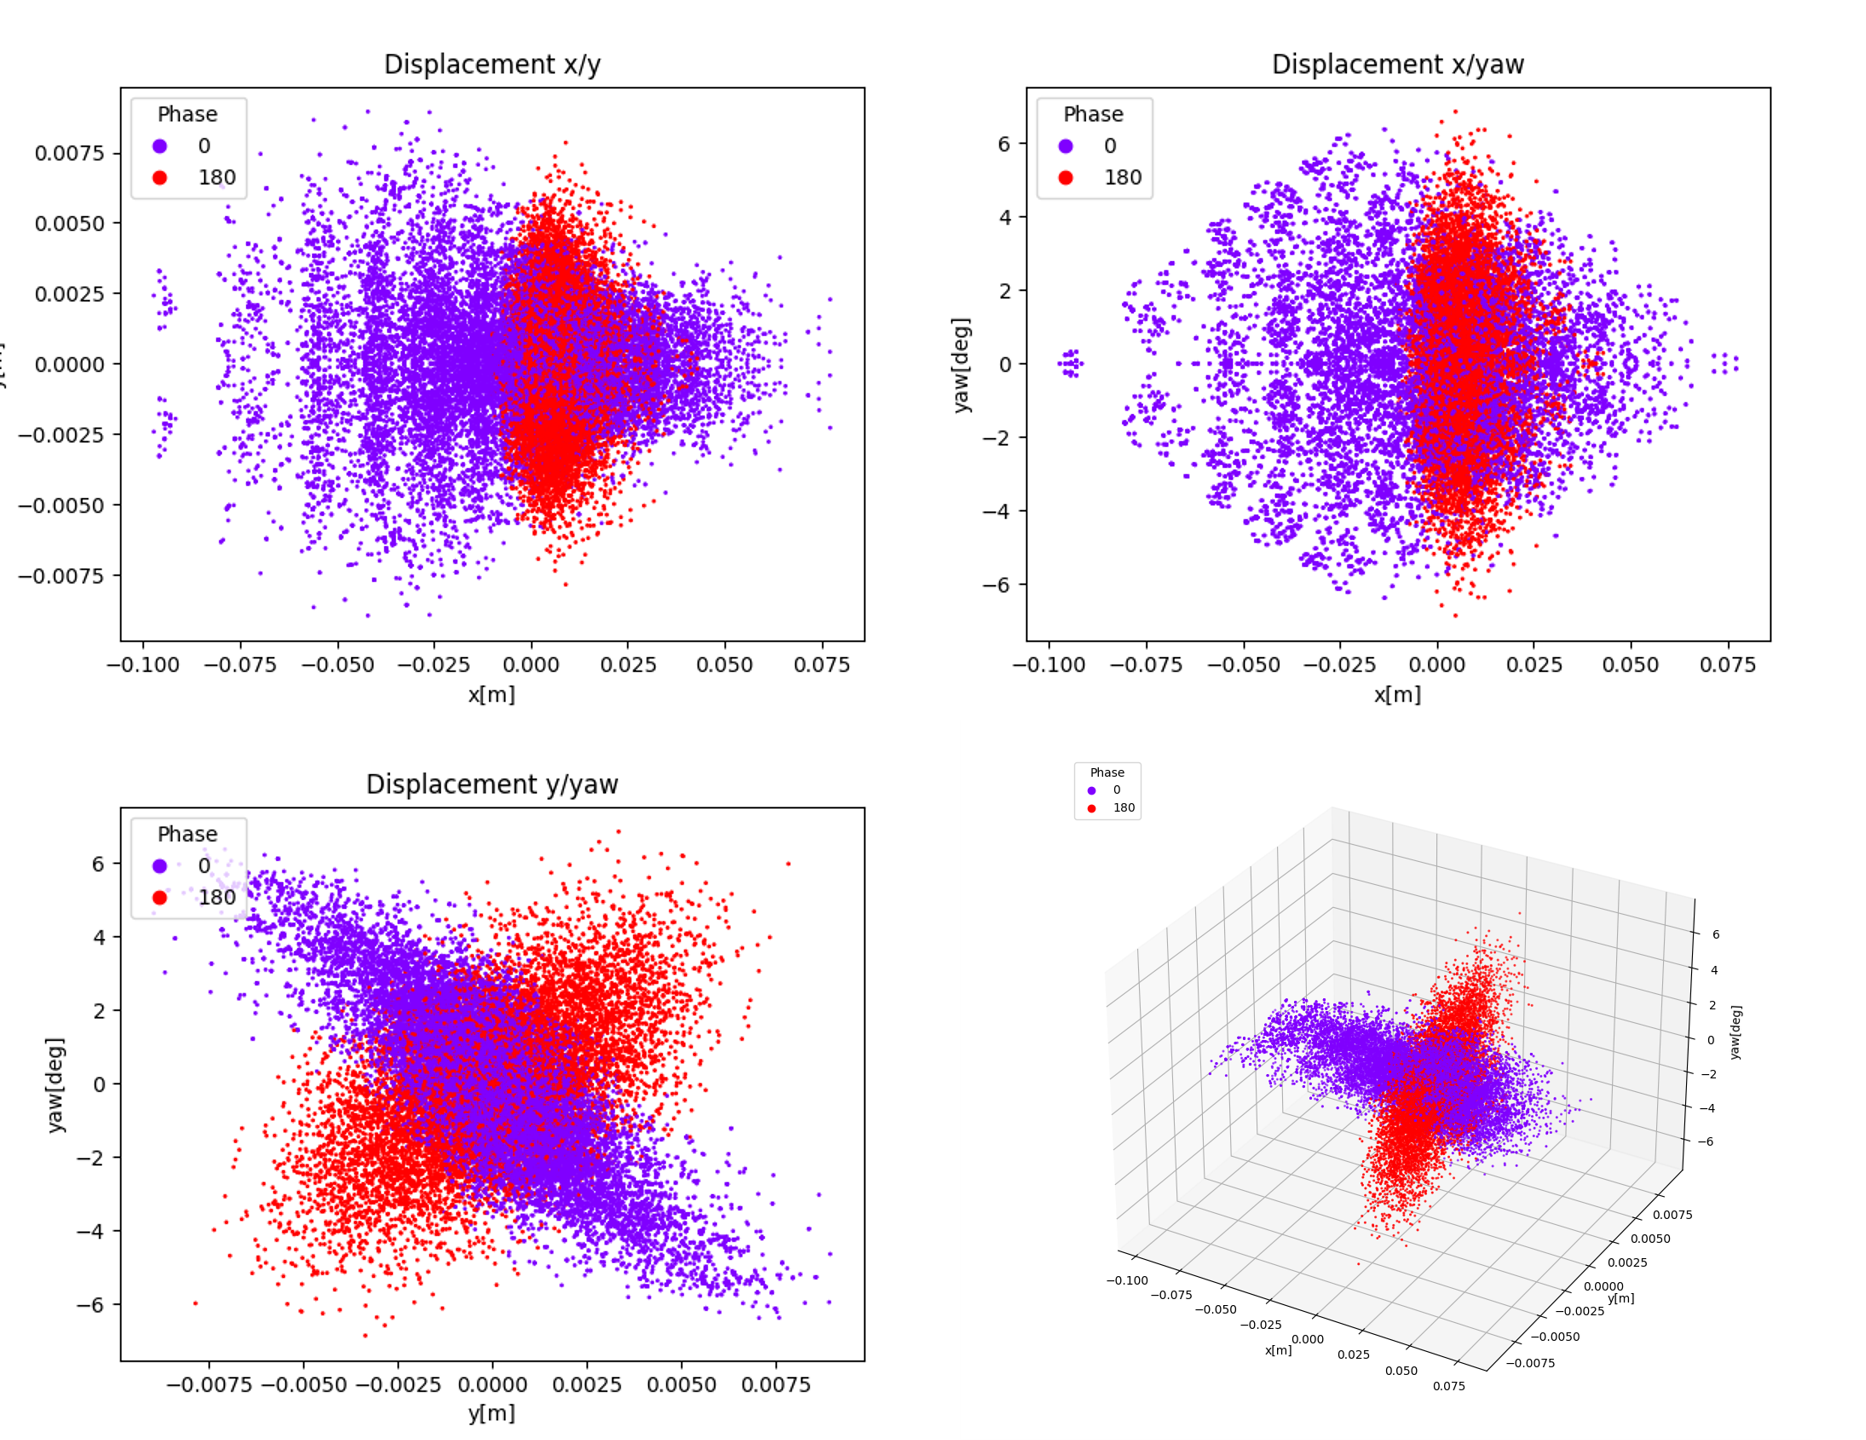
\includegraphics[width=0.66\textwidth]{images/displacement_spread.png}
            \caption{Multiple view of the possible motion of the robot. The robot can move along x-axis and y-axis, but also change its orientation. Bottom right plot shows the 3D view of the $40'000$ possible sequences. Other plots are a projection of those point on only 2 axis. Red dots are sequences with a 180° phase difference while purple dots are sequences with no phase difference.}
            \label{fig:displacement_spread}
        \end{figure}
        
        Figure \ref{fig:displacement_spread} shows the spread of displacement and orientation for the $40'000$ different sequences (A-J). There are two different color depending on the phase difference applied. Red dots represent a phase difference of 180°, corresponding to the actuators extending and retracting in opposition.
        
    \section{Deep Q Learning Results}\label{sec:res_qlearning}
        The Deep Q Learning controller is able to learn how to select sequences to drive the robot to a specific place given a current state. Figure \ref{fig:dqn_results} shows an example of learning process for a robot restricted to use only sequences A and B for each leg. On the Figure, a plateau is created after 40 iterations where the number of steps stabilize around 200 and the number of sequence switch for the scenario stabilize around 35. The results also include multiple videos where the controller is shown in action and complete the tasks successfully.
        \begin{figure}[h]
            \centering
            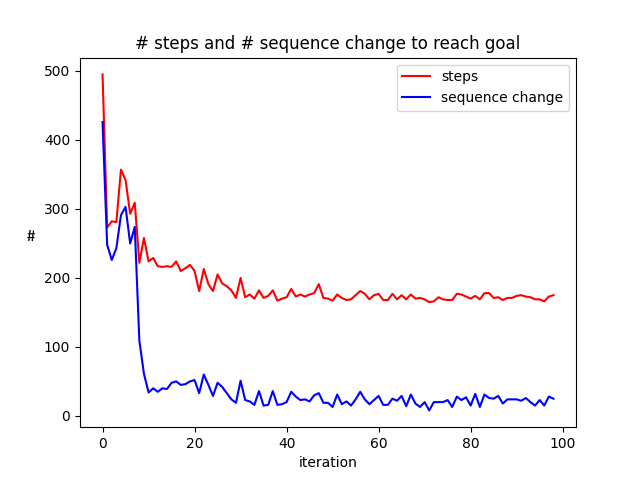
\includegraphics[width=0.7\textwidth]{images/AB-0-FALSE.png}
            \caption{Learning process of a Deep Q Learning Controller. Two lines are plotted and represent the progression, red line is the number of steps done for each iteration to reach the goal. The blue line represents the number of sequence switch that occur during the iteration. Each iteration consist of the same scenario but with different starting orientations (which is the end orientation of the previous scenario). The robot was restricted to use only sequences A and B.}
            \label{fig:dqn_results}
        \end{figure}
        
        Figure \ref{fig:all_sequences} shows the learning progress of a similar Deep Q Learning (two layer of hidden layers instead of one), but instead of restricting to some sequences, the neural net is given all the possible sequences. Again the red line represent the number of steps required for the iteration and the blue line represent the number of switches.
        
        \begin{figure}
            \centering
            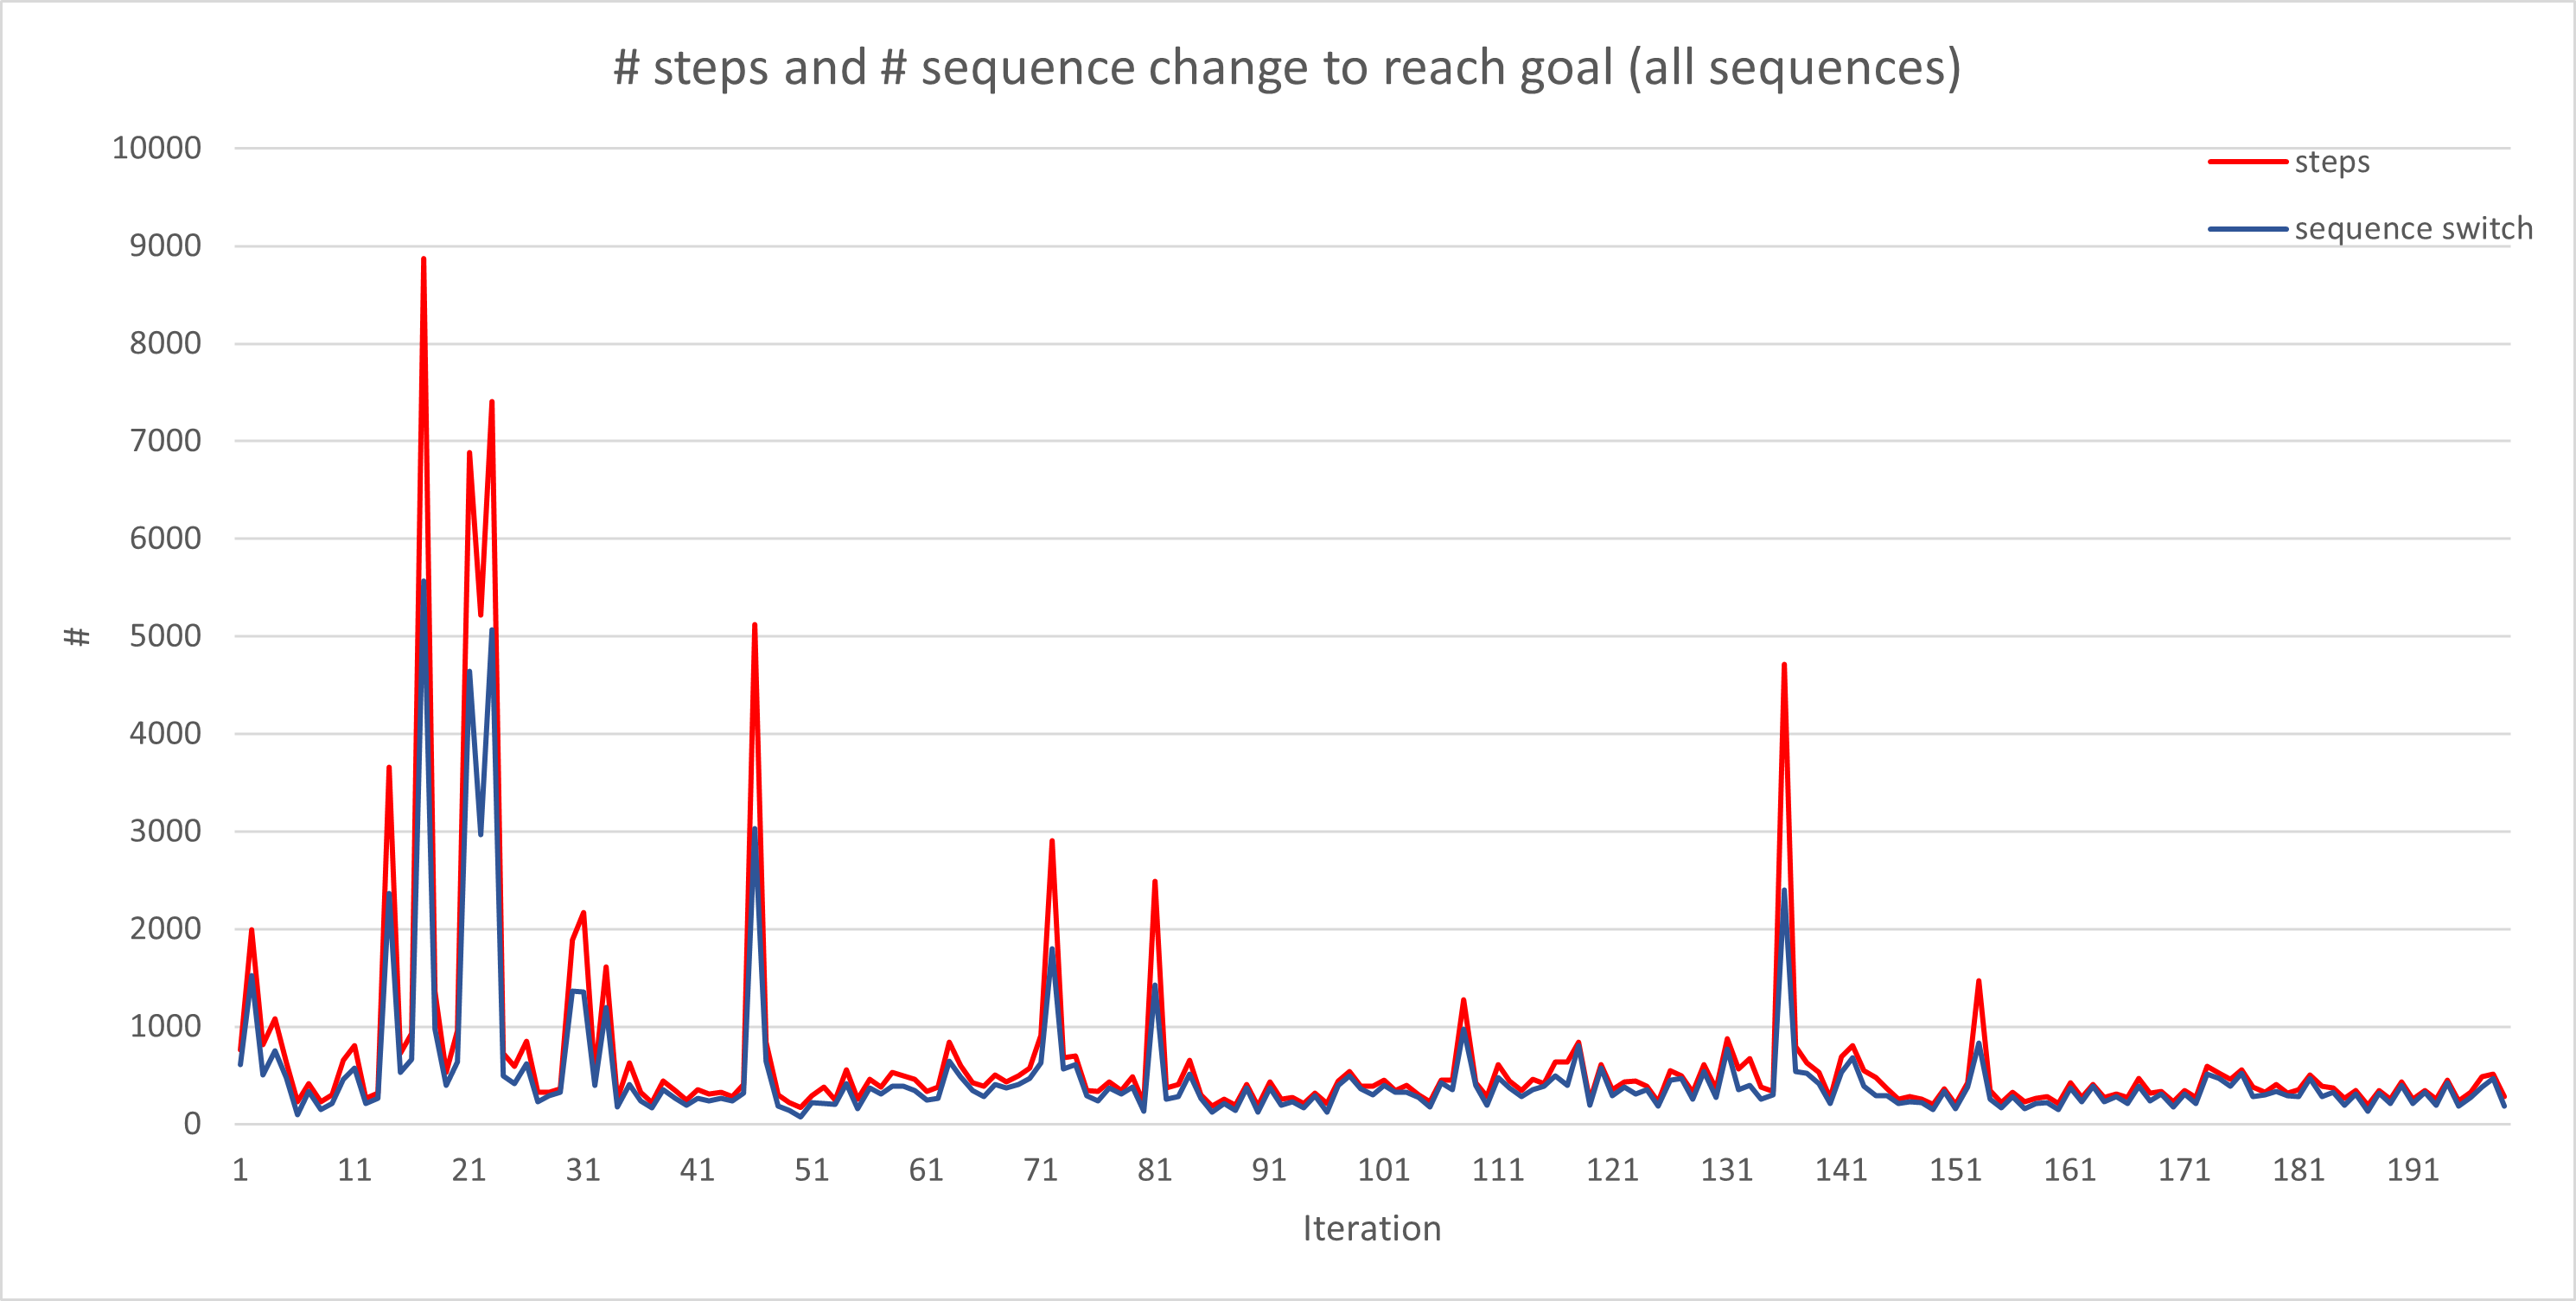
\includegraphics[width=0.9\textwidth]{images/ALL_SEQ_QLEARN.png}
            \caption{Example of Deep Q Learning process with all the sequences enabled. Red line represent the number of steps to reach to the iteration target. Blue line represent the number of sequence changes done during the iteration.}
            \label{fig:all_sequences}
        \end{figure}
        